\documentclass{article}
\usepackage{v-problem}
\vgeometry

\begin{document}
\vtitle[KINEMATICS]

\def\pn{05}
\def\book{A.K.}
\def\page{28}
\def\gdrive{https://drive.google.com/drive/folders/1a14eiGsMZ_QecLcubMDaiyEv27izH7XV?usp=share_link}

\def\question{
A boat is rowed with constant velocity $u$ starts from point $A$ on the bank of a that river of width $d$, which flows at a constant speed $nu$; it points always towards a point $O$ on the other bank exactly opposite to $A$. Find the path equation $r = f(\theta)$ for the boat.
}

\def\option{
}


\begin{tikzpicture}
	\node[qnumber] (n) at (0, 0)[scale=2] {$\pn.$};
	\node[question] (q) [right=2mm of n.east] {\question};
	\tzline[divider]<-0.125, 0> (q.north west)(q.south west);
	\node[format] (f) at  (q.south east){[\book \quad \page]};
	%\node[diagram] (d) [below=1cm of q.south] {\diagram};
	%\node[option] (o) [below=0.1cm of d.south] {\option};
\end{tikzpicture}	
\vspace*{\fill}

\begin{center}
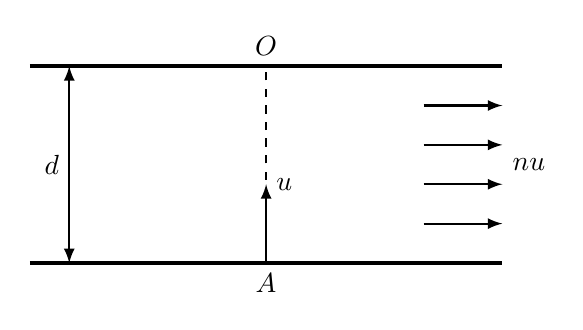
\begin{tikzpicture}
[>=latex, thick]
%\draw[->] (0, 0)--((5, 0);
%\fill[pattern=north east lines](0, 0) rectangle (4, -0.5);
\draw[ultra thick] (-3, 0)--(3, 0) (-3, 2.5)--(3, 2.5);
\foreach \y in {0.5, 1.0,..., 2}{
\draw[->] (2, \y)--(3, \y);
};
\node at (3, 1.25)[right]{$nu$};
\draw[dashed](0,0)--(0, 2.5) node[above]{$O$};
\draw[->](0, 0) node[below]{$A$}--+(0, 1) node[right]{$u$};
%\draw (0, 0.3) arc (90:135:0.3);
\draw[<->](-2.5, 0)--(-2.5, 2.5) node[left, midway]{$d$};
\end{tikzpicture}
\end{center}
\vspace*{\fill}
\pagebreak
\vtitle[\texttt{SOLUTION}]

\begin{center}
\begin{tikzpicture}
[>=latex, thick]
\tzcoor*(0,  0)(A){$A$}[b]
\tzcoor*(0,  3)(O){$O$}[a]
\tzline[ultra thick]($(O)+(-3.5, 0)$)($(O)+(3.5, 0)$)
\tzline[ultra thick]($(A)+(-3.5, 0)$)($(A)+(3.5, 0)$)

%\foreach \y in {0.5, 1.0,..., 2.5}{
%\tzline+[->] (2.75, \y)(1, 0);
%};
%\node at (3.75, 1.5)[right]{$v=nu$};
\tzline[dashed](A)(O)

\tzline[<->]<-3, 0>(A)(O){$d$}[left, midway]
\tzto[out=0, in=-120]"path"(0, 0)(1.5, 1.2);
\tzvXpointat{path}{1.5}(P){$P(r, \theta)$}[l]

\tzline[dashed]($(P)!0.5!(O)$)(O)
\tzline[->](P)($(P)!0.5!(O)$){$u$}[bl]
\tzline+[->](P)(1.2, 0){$v=nu$}[r]
\tzline[->, dashed](P)($(P)!-0.45!(O)$){$v\sin\theta$}[r]
\tzline[->](P)($(P)!0.5!-90:(O)$){$v\cos\theta$}[r]
\tzdot*(P)(4pt)

\tzanglemark(A)(O)(P){$\theta$}(12pt)
\tzanglemark($(P)+(1, 0)$)(P)($(P)!0.5!-90:(O)$){$\theta$}(12pt)

\end{tikzpicture}
\end{center}

$OP(r)$ is being covered by relative velocity along the line also the angle($\theta$) is changing by the tangential velocity($v\cos\theta$). So, we can write following differential equations.

\addtolength{\jot}{3ex}
\begin{align}
-\dfrac{\d{r}}{\d{t}} &= u - v\sin\theta \\
r\dfrac{\d{\theta}}{\d{t}} &= v\cos\theta
\end{align}
\pagebreak

By dividing equation (1) and (2), then integrating with proper limits\_ 

\begin{align*}
-\dfrac{\d{r}}{r} &= \dfrac{u-v\sin\theta}{v\cos\theta} \d{\theta}\\
-\int_d^r \dfrac{\d{r}}{r} &= \int_0^\theta \dfrac{u}{v}\sec\theta \d{\theta}- \int_0^\theta \tan\theta \d{\theta}\\
-\ln r \bigg\rvert_d^r &= \dfrac{1}{n} \ln \left(\tan\left(\dfrac{\theta}{2} + \dfrac{\pi}{4} \right)\right)-\ln\sec\theta \bigg\rvert_0^\theta\\
\ln\left(\dfrac{r}{d}\right) &= \ln\left(\dfrac{\sec\theta}{\left[ \tan\left(\dfrac{\theta}{2} + \dfrac{\pi}{4} \right) \right]^{1/n}}\right) \\
r &= \dfrac{d\sec\theta}{\left[ \tan\left(\dfrac{\theta}{2} + \dfrac{\pi}{4} \right) \right]^{1/n}} \ans
\end{align*}

\pagebreak

\vspace*{\fill}
\begin{center}
	\fbox{\qrcode[height=2cm]{\gdrive}}
\end{center}
\vspace*{\fill}

\end{document}
